\documentclass{article}
\usepackage{a4wide}
\usepackage[utf8]{inputenc}
\usepackage[T1]{fontenc} 
\usepackage{fancyhdr} 
\usepackage{graphicx}
\usepackage{lastpage}
\usepackage{enumerate}
\usepackage{amssymb}
\usepackage{amsmath} 
\usepackage{algorithm}
\usepackage{tikz} 
\usepackage{listings}
\usepackage[noend]{algpseudocode}
\usetikzlibrary{automata, arrows}
\usepackage{subcaption}
\usepackage{hyperref}
\usepackage{booktabs}

\makeatletter
\def\BState{\State\hskip-\ALG@thistlm}
\makeatother



\lhead{
\includegraphics[width=4.6cm]{uni.png}\\ \course\\ \semester\\Segmentation of Femurs \homeworkNumber}
\rhead{\university\\ \authorname\\\authoremail\\Page \thepage\ of \pageref{LastPage}}

\usepackage[headheight=68pt]{geometry}
\pagestyle{fancy}

%% Custom command
\newcommand{\authorname}{Giorgi Grigalashvili, Fabricio Arend Torres}
\newcommand{\authoremail}{\{g.grigalashvili, fabricio.arendtorres\} @ stud.unibas.ch}
\newcommand{\semester}{Spring Semester 2017}
\newcommand{\course}{Probabilistic Shape Modelling}
\newcommand{\homeworkNumber}{}

\newcommand{\university}{University of Basel}
\newcommand{\department}{Department of Mathematics and Computer Science}
\newcommand{\address}{Spiegelgasse 1, 4051 Basel, Switzerland}
\newcommand{\website}{dmi.unibas.ch / informatik.unibas.ch}

%% Custom commands

\def\underline#1{\underline{\underline{#1}}}

\begin{document}
	\author{Giorgi Grigalashvili, Fabricio Arend Torres}
		\title{Project 2:\\ Femur Segmentation from CT Scans}
	\maketitle
	\begin{abstract}
		In this second project, we implemented a sampling procedure that allows us to automatically segment femurs from CT scans by using a provided active shape model.
		The basic idea relies on the combination of a pixel intensity model and a statistical shape model.
		Through MCMC sampling it is possible to estimate an optimal fit in terms of the posterior probability of the model given the CT scan in form of a '.nii' image.
	\end{abstract}
	

	\section{Introduction}
	Automated image segmentation in the medical field poses a difficult problem which could significantly improve many processes.
	The difficulty arises due to partial volume effects, artifacts in the image and general noise.
	The aim of the project is the segmentation of 5 femurs, for each of which a CT scan image is provided. 
		
	The approach presented in this paper relies on an active shape model for femurs, which is a combination of a statistical shape model and an intensity model.
	The Shape Model provides a probability distribution over femur shapes, which was presumably learned from observed data.
	The intensity model models the intensities at areas around given profile points of the shape model.	


	\section{Method}
	Our aim is finding a femur shape defined by the parameter set $\theta$ which explains the image intensities observed in the CT as good as possible while still considering realistic and likely femur shapes.
	More formally we search for:
	\begin{equation}
	\theta* = \arg\max_\theta \frac{p(\theta) P(I_T | \theta)}{\int p(\theta) p(I_T | \theta) \delta\theta}
	\end{equation}	
	
	The used ASM models the image intensities as normal distributions for specific profile points, which lie orthogonal to the shapes.
	The mean intensities are visualized in \autoref{1.1}.
	In the segmentation procedure we can use this for evaluating the likelihood for observing intensities at the position of the profile points for a specific shape instance.
	\begin{equation}
	p(I_T (h_\theta (x_i)) | \theta,x_i ) = \mathcal{N}(\mu_i, \Sigma_i) 
	\end{equation}
	where $\theta$ is a possible set of parameters that defines an instances of the shape model.
	
	By assuming that the noise at the different profile points are independent and identically distributed, we can calculate the total likelihood of an image by taking the product of the likelihoods.
	
	
	\begin{equation}
	p(I_T(h_\theta (x))|\theta, \Gamma_R) = \prod_{i} \mathcal{N}(\mu_i, \Sigma_i)
	\end{equation}
	
	
	
	\begin{figure}
		\centering
		%\begin{subfigure}{.5\textwidth}
			\centering
			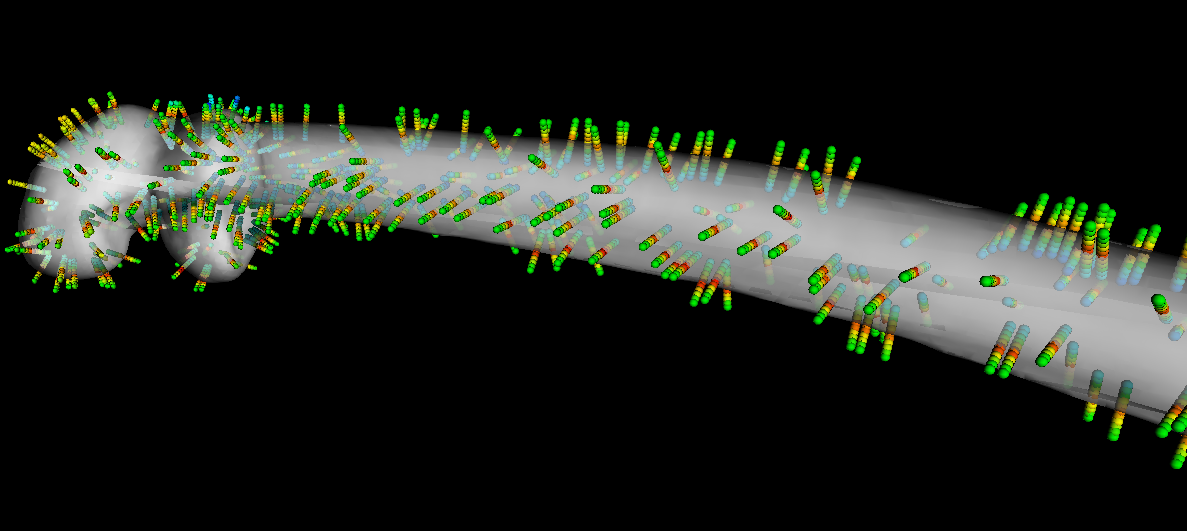
\includegraphics[width=0.8\textwidth]{images/mean_pixelintensities.png}
			\caption{Mean Intensities and mean shape of the ASM}
			\label{1.1}
		%\end{subfigure
	\end{figure}	
	\begin{equation}
	Q(\theta' | \theta) = N(\theta'|\theta, \Sigma_\theta)
	\end{equation}
	\begin{equation}
	u = \mu + \sum_{i=1}^\infty \sqrt{\lambda_i} \phi_i \alpha_i, \quad \alpha_i \sim{} \mathcal{N}(0,1)
	\end{equation}
	\begin{equation}
		\alpha = min \{ \frac{P(\theta' | D ) Q(\theta|\theta')}{P(\theta|D) | Q(\theta'|\theta)}, 1\}
	\end{equation}
	\begin{center}
		\begin{tabular}{l l l l l}
			\toprule
			update type & $\sigma$ & Probability \\
			\midrule
			Batch Random Walk $N(0, \Sigma)$&  0.001 & 	0.2  	\\
			Batch Random Walk $N(0, \Sigma)$& 0.01 & 	0.4 	\\
			Batch Random Walk $N(0, \Sigma)$& 0.05 &	0.2		\\
			Batch Random Walk $N(0, \Sigma)$& 0.2&		0.2		\\
			Single Parameter Random Walk $N(0,\sigma_i)$ & 0.1& $\frac{1}{rank(ShapeModel)}$
		\end{tabular}
	\end{center}
	\section{Problems}
	
	\section{Results \& Discussions}
		\begin{figure}
			\centering
			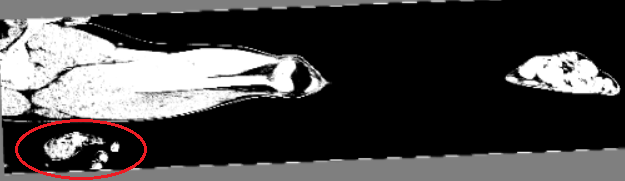
\includegraphics[width=0.9\textwidth]{images/CT_10_foot.png}
			\caption{Artifacts in the CT scan: another foot}
			\label{2.1}
		\end{figure}		
		\begin{figure}
			\centering
			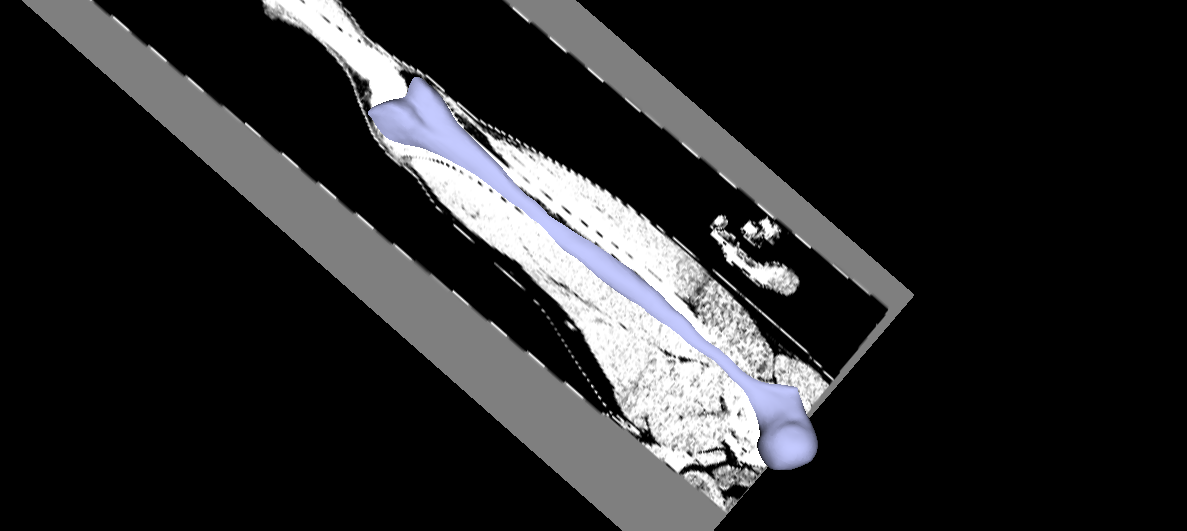
\includegraphics[width=0.9\textwidth]{images/segmentation_10_outofrange.png}
			\caption{Possible Variations may be out of range of the CT image}
			\label{2.2}
		\end{figure}
	


\end{document}